\newpage
\section{Implementierung}

\subsection{Treiber}
Als Treiber für die H-Brücke wird der A3941 von Allegro Microsystems 
verwendet. Dieser Chip ist bei Farnell für ca. 8 CHF verfügbar und bietet eine 
einfache DC-Motorenansteuerung mittels PWM-Signal und Richtungsangabe.

\subsubsection*{Eckdaten zum A3941 Treiberchip}
\begin{itemize}
	\item Betriebsspannung: 5.5 – 50\si{\volt}
	\item Geschwindigkeitseinstellung mittels PWM
	\item Richtungsbestimmung
	\item Preis: ca. 8 CHF
	\item Externe H-Brücke
\end{itemize}

\subsection{Timer}
Dieser Teil der Schaltung erzeugt das interne PWM-Signal. Mithilfe des
NE555 wird ein Sägezahnsignal erzeugt, welches auf den Komparator in IC1
geführt wird. Dieser vergleicht diesen Sägezahn mit dem Schwellwert,
welcher mit dem Potentiometer R7 oder den beiden Widerständen R22 und R23
eingestellt werden kann (R22 und R23 sind eine Bestückungsvariante). 
Sobald der Sägezahn über dem Schwellwert ist, gibt der Komparator eine Spannung 
von 15\si{\volt} aus. Wenn der Sägezahn tiefer ist zieht er seinen Ausgang 
auf Ground. Da er einen Open-Drain Ausgang hat, benötigt er einen Pull-Up 
Widerstand am Ausgang.

\begin{figure}[h!]
	\centering
	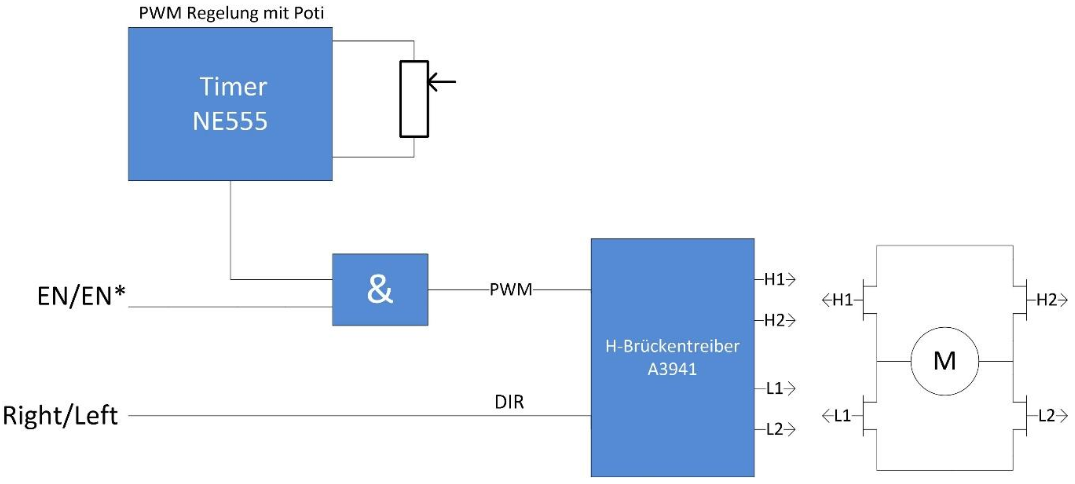
\includegraphics[width=0.75\textwidth]{src/dc/fig/timer_block.png}
	\caption{Blockschaltbild der Timerschaltung}
\end{figure}

\begin{figure}[h!]
	\centering
	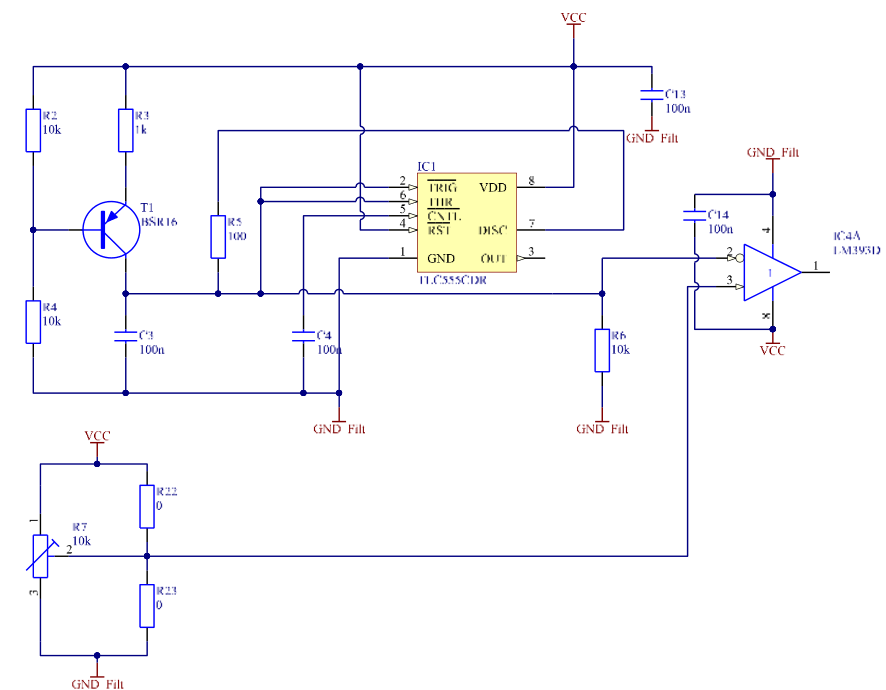
\includegraphics[width=0.75\textwidth]{src/dc/fig/timer_schematic.png}
	\caption{Timerschaltung}
\end{figure}

\newpage
\subsection{PWM-Logik}
Mit dieser Logik kann ausgewählt werden, ob das interne oder ein externes
PWM Signal verwendet wird. Wird auf das Switch-Signal eine logische
0 gelegt, wird das interne PWM verwendet, bei einer logischen 1 das externe
PWM. Das Switch Signal kann auch als ON/OFF Signal für das interne PWM
verwendet werden. Dazu muss nur das externe PWM Signal dauerhaft auf Ground
geschaltet werden. Auf diese Art kann zwischen internem PWM und keinem PWM
umgeschaltet werden. Diese Betriebsart wird im Moment verwendet.

\noindent
Die Zehnerdiode am Ausgang wird benötigt, um das Ausgangssignal auf den
Logikpegel des A3941 zu senken. Die 4xxx IC Reihe kann mit bis zu 18\si{\volt} 
betrieben werden und gibt auch annähernd diese Spannung wieder aus. Da der 
A3941 einen maximalen Logikpegel von 6.5\si{\volt} verträgt, muss die 
Signalspannung reduziert werden.

\begin{figure}[h!]
	\centering
	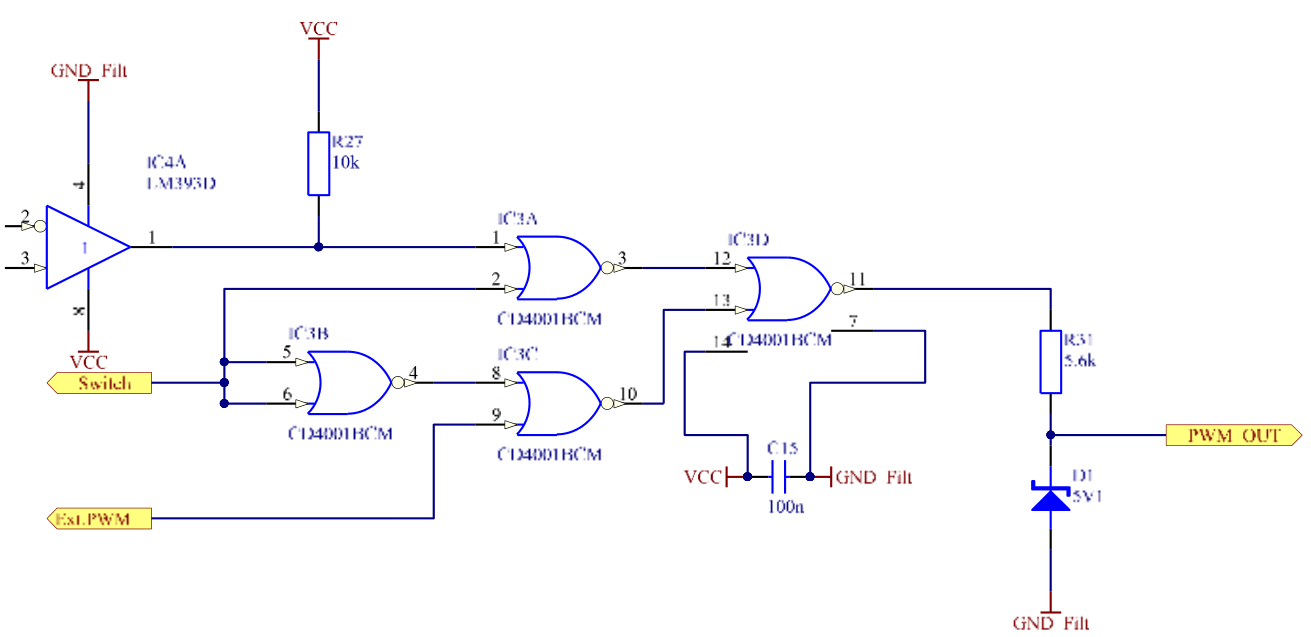
\includegraphics[width=0.75\textwidth]{src/dc/fig/pwm_schematic.png}
	\caption{PWM-Logik}
\end{figure}

\subsection{Ansteuerung}

\begin{figure}[h!]
	\centering
	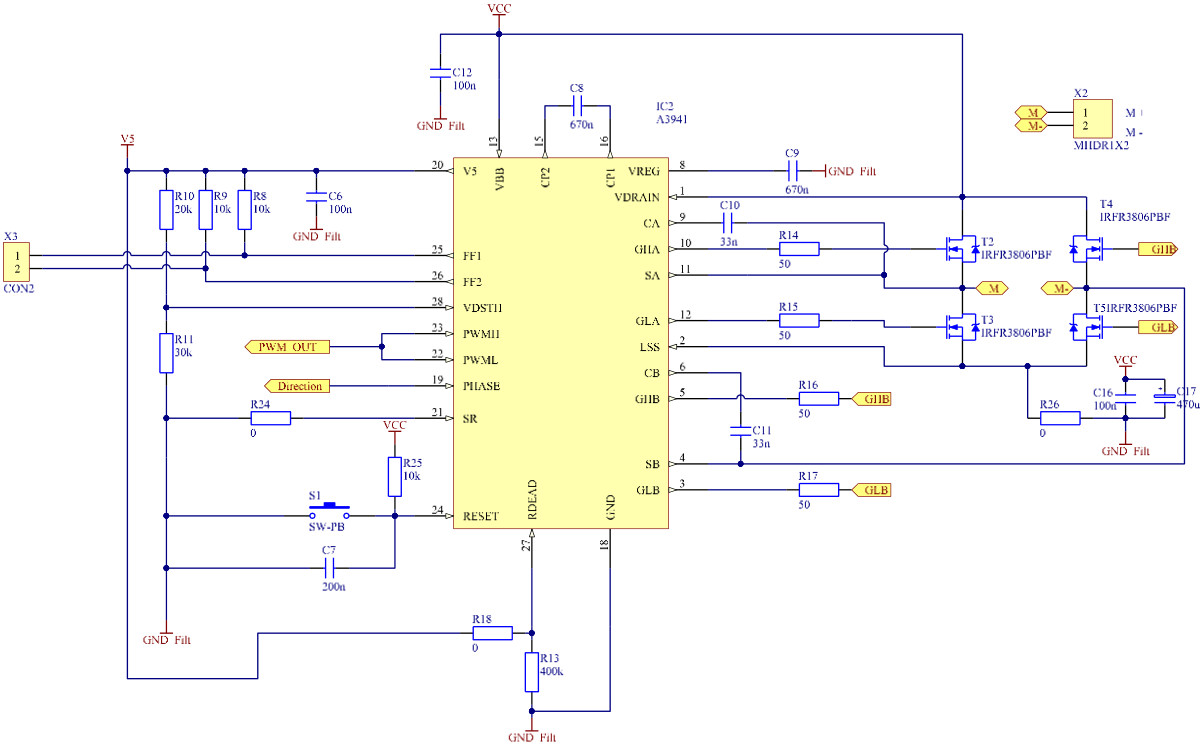
\includegraphics[width=0.75\textwidth]{src/dc/fig/driver_schematic.png}
	\caption{Treiberschaltung}
\end{figure}

\noindent
Mit dem Phase-Eingang kann die Richtung eingestellt werden. Bei PWMH und
PWML wird das PWM Signal angeschlossen. Der Motorentreiber wird im
Fast-Decay Modus betrieben. Das heisst, die Spule des Motor wird beim
Abbremsen über die Dioden der H-Brücke entladen.

\begin{figure}[h!]
	\centering
	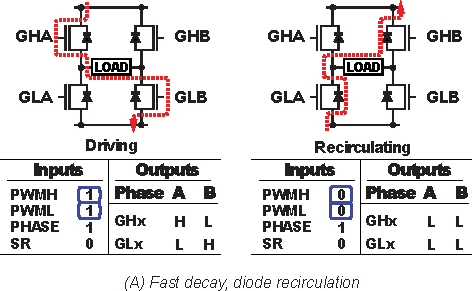
\includegraphics[width=0.5\textwidth]{src/dc/fig/decay.pdf}
	\caption[Fast Decay Illustation]{Fast Decay Illustation \cite{Datasheet:A3941}}
\end{figure}

\subsubsection{Ladungspumpe}
Die Ladungspumpe (Charge-Pump) wurde anhand des Datenblattes des A3941
und der eingesetzten MOSFET berechnet und eingesetzt. Die dazu notwendige
Kapazität ist wie folgt berechnet:

\[  
	C_{BOOT}
		= \frac{20 \cdot Q_{GATE}}{V_{BOOT}}
		= \frac{20 \cdot 30\mathrm{nC}}{10\mathrm{V}}
		= 33.3\mathrm{nF} 
		\xrightarrow{E6} 33\mathrm{nF}
\]

\noindent
Die Stützkapazität ist mit dem 20-fachen Wert zu belegen, also mit:
\[
	C_{REG}
		\approx 20 \cdot C_{BOOT}
		= 20 \cdot 33\mathrm{nF}
		= 660\mathrm{nF}
\]
